% !TeX encoding   = UTF-8
\documentclass[12pt]{article}

\usepackage{sbc-template}

\usepackage{graphicx,url}
\usepackage[brazil]{babel}
\usepackage[utf8]{inputenc}
\usepackage{graphicx}   %Package para figuras
\usepackage{enumerate}
\usepackage{tabularx}
\usepackage{multirow}
\usepackage[table,xcdraw]{xcolor}
\usepackage{todonotes}

\sloppy

\title{Um estudo sobre o efeito de Mover Classe na Arquitetura de Sistemas}

\author{Vagner Clementino\inst{1}}

\address{Departamento de Ciência da Computação\\
        Universidade Federal de Minas Gerais (UFMG)\\
  \email{vagnercs@dcc.ufmg.br}
}

\date{Maio de 2016}
\begin{document}

\maketitle

\begin{resumo}
 Recentemente estudos vêm focando em entender as motivações que levam os desenvolvedores a realizem refatoração do código. Existe um consenso que a causa original é remover porções de código com baixa qualidade conhecidos como \textit{Bad Smells}. Todavia, estudos demonstraram que o desenvolvedores refatoram para outros fins. Neste sentido, este trabalho se propõe em analisar a relação entre mudanças na arquitetura de um sistema e a refatoração \textit{Mover Classe}. Após a análise de 52 mil commits de 04 sistemas de código aberto hospedados no GitHub verificou-se em todos o fenômeno de \texttt{batching moving}, que é movimentação substancial de classes dentro do sistema. Este evento tem impactos na arquitetura do software.
\end{resumo}


\section{Introdução}
\label{sec:intro}

A atividade de refatoração tem por objetivo alterar o código fonte de um software sem modificar o seu comportamento. Em última instância, refatorar visa melhorar a qualidade interna do sistema \cite{Fowler1999,Opdyke:1992:ROF:169783}. Sua importância é reconhecida tanto na literatura quanto na indústria, no qual, nesta última, é possível verificar a existência de processos de desenvolvimento que incorporam a refatoração como atividade rotineira \cite{Beck:2000:PEP:557458}. No últimos anos, pesquisas foram realizadas com o objetivo de entender com qual frequência os desenvolvedores aplicam diferentes tipos de refatoração \cite{Murphy-Hill:2009:WRW:1555001.1555044}; a relação entre a atividade de refatorar e a correção de \textit{bugs}\cite{Kim:2011:EIR:1985793.1985815}, bem como nos resultados de testes de regressão  \cite{Kim:2012:EII:2473496.2473590}. No trabalho de kim et.al discute a percepção dos desenvolvedores sobre a refatoração \cite{Kim:2012:FSR:2393596.2393655}.

Recentemente estudos vêm focando em entender as motivações que levam os desenvolvedores a realizem refatoração. Existe um consenso que a causa original é remover porções de código com baixa qualidade conhecidos como \textit{Bad Smells} \cite{Fowler1999}. Todavia, estudos demonstraram que o desenvolvedores refatoram para outros fins. Por exemplo, a refatoração \textit{Extrair Método}, pode ser utilizada para fins de extensão do sistema ou mesmo possibilitar compatibilidade com versões anteriores do código \cite{Tsantalis2013}. É possível verificar o emprego de \textit{Extrair Método} com intuito de favorecer a reutilização de código no longo prazo, mesmo que inicialmente não seja esta a intenção \cite{Danilo}.

Apesar da existência de estudos relativos à motivação da refatoração, ao bem do nosso conhecimento, não existem trabalhos que relacionem a refatoração \textit{Mover Classe} com mudanças na arquitetura do sistema. Suspeitamos que o fato de um desenvolvedor mover classes em um número maior que padrão do sistema tem por objetivo alterar a arquitetura do sistema. Este tipo de ação é conhecida como \texttt{batching moving}. Uma alteração na arquitetura pode ter como objetivo, por exemplo, reorganizar o código existente em uma nova camada lógica ou ainda tratar o problema da  \textit{Erosão Arquitetural}. O processo de Erosão arquitetural é conhecido como os desvios ocorridos no código de um sistema que causam violação de alguma regra arquitetural previamente estabelecida \cite{Perry:1992:FSS:141874.141884}.

Neste sentido, este trabalho se propõe em analisar a relação entre mudanças na arquitetura de um sistema e a refatoração \textit{Mover Classe}. A fim de investigar tal relação analisamos o histórico de versões de 04 sistemas de código aberto, desenvolvidos em Java e hospedado no \texttt{GitHub}. Este estudo visa responder a seguinte questão de pesquisa:

\begin{description}
	\item[RQ] Com qual frequência a refatoração Mover Classe tem por objetivo alterar a arquitetura do sistema (\texttt{batching moving})?	
\end{description}

Ao responder a questão proposta entendemos que iremos contribuir no aumento do entendimento das razões que levam os desenvolvedores a realizar refatorações. Esta informação poderá ser utilizada posteriormente na construção de ferramentas que ajudem os times de desenvolvimento em tarefe relativas à mudança da arquitetura do software. Além disso será possível verificar a relação entre a atividade de refatoração e a mudança de arquitetura de um sistema. 

O restante deste trabalho está organizado da seguinte forma: a Seção \ref{sec:metodologia} descreve a metodologia utilizada neste estudo; a Seção \ref{sec:resultados} apresenta os resultados e responde a questão de pesquisa; na Seção \ref{sec:ameacas} realiza-se uma discussão sobre as ameaças à validade do trabalho; a Seção \ref{sec:trabalhos-relacionados} apresenta os trabalhos relacionados à análise da atividade e detecção de refatoração; a Seção \ref{sec:conclusao} sumariza o artigo e discute suas principais contribuições.

\section{Metodologia}
\label{sec:metodologia}


\subsection{Seleção dos Sistemas}
\label{subsec:selecao_sistemas}

Com o objetivo de responder as questões de pesquisa propostas neste trabalho foram coletados sistemas de código aberto hospedados no \textsl{GitHub}. Com cerca de 38 milhões de repositórios\footnote{\url{https://github.com/features}. Acesso em junho/2016.}, GitHub é atualmente o maior repositório de código na Internet. Sua popularidade e a disponibilidade de metadados, acessíveis através de uma API, tem tornando GitHub bastante atrativo para a realização de pesquisas na área de Engenharia de Software. 

Para escolha dos projetos foi definido inicialmente um conjunto de critérios baseados em boas práticas recomendadas na literatura \cite{Bird2009}. Em síntese, um projeto para ser escolhido deve atender aos simultaneamente seguintes requisitos:

\begin{itemize}
	\item Os projetos devem ter Java como a linguagem principal, por limitações da
ferramenta de analise utilizada.
\\
	\item Os projetos devem ter no mínimo seis meses de desenvolvimento, para evitar projetos que não 
tenham passado por um tempo de manutenção relevante.
\\
\item Os  projetos  devem  ter  no  mínimo  200  revisões  pelos  mesmos  motivos  da
restrição anterior.
\\
\item Os projetos escolhidos não devem ser ramificações (\textsl{forks}) um do outro projeto, para evitar dados duplicados.

\item Os projetos obtidos devem ser os 120 mais populares que atendem aos demais critérios, utilizando como métrica o campo \texttt{most stars}
\end{itemize}

Os projetos foram recuperados através a busca avançada do GitHub\footnote{\url{https://github.com/search/advanced}} utilizados os critérios:  \textsl{created:}$<2016-01-01$ \& \textsl{language:Java}. O resultado foi ordenado pelo parâmetro \textsl{"Most stars"} até o limite de 120 projetos. Ao conjunto recuperado foi aplicado os critérios de escolha definidos previamente. Ao final do processo foram escolhidos os projetos descritos na Tabela \ref{tab:projetos}. 

\textsl{JUnit} é um \textit{framework} para escrever testes. O \textsl{Spring Framework} fornece um modelo de programação para aplicações empresariais baseadas em Java. \textsl{Clojure} é uma linguagem de programação de propósito geral com tipagem dinâmica. \textsl{Gradle} é uma ferramenta de \texttt{build} com foco na automação e suporte a multilinguagem. O conjunto selecionado abrange diversos tipos de sistema, desde de linguagens de programação, passando por \textit{frameworks} de teste e desenvolvimento até chegar em ferramenta de \texttt{build}. Trata-se de sistema bem conceituados dentro do seu campo de atuação.

\begin{table}[htb]
	\centering
	\resizebox{\textwidth}{!}{%
		\begin{tabular}{|c|c|c|c|c|}
			\hline
			\textbf{Projeto}          & \textbf{Commits} & \textbf{Branches} & \textbf{Releases} & \textbf{Contribuidores} \\ \hline
			\textit{junit4}           & 2105             & 5                 & 20                & 123                     \\ \hline
			\textit{spring-framework} & 12178            & 10                & 89                & 160                     \\ \hline
			\textit{clojure}          & 2953             & 22                & 100               & 124                     \\ \hline
			\textit{gradle}           & 36947            & 50                & 829               & 227                     \\ \hline
		\end{tabular}%
	}
	\caption{Projetos Analisados. Os dados apresentados tem como referência 22/06/2016.}
	\label{tab:projetos}
\end{table}


\subsection{Detecção das Refatorações}
\label{subsec:deteccao_refatoracoes}

%\subsubsection{Detecção do Mover Classe}

Para que fosse possível detectar a presença de \texttt{batching moving}, ou seja, de um conjunto de movimentações de classes em um número maior do que o padrão do sistema, se fez necessário detectar a refatoração \textit{Mover Classe}. Com este objetivo, cada alteração de código existente no histórico de versões do sistema foi analisada. 

Um problema que surge quando se analisa revisões consecutivas de um sistema, em especial para aqueles que utilizam um sistema de controle de versão distribuído, como é o caso do \texttt{git}, é o \textit{implicit branches}{}. Quando dois desenvolvedores que colaboram no mesmo projeto realizam alterações locais pode ocorrer que ambos repositórios divirjam. No caso de um futuro \textit{merge}{} que contenha pelo menos dois pais pode resultar duplicação das refatorações detectadas, caso a atividade de refatoração tenha ocorrido em pelo menos um dos \textit{branches}{}. A  Figura \ref{fig:implicit_brache} exibe uma sequência de \textit{commits} ilustrando o problema da da duplicação da contagem de refatorações. Suponhamos que exista um \textit{refactoring} em $c_4${}. Ele será detectado quando compararmos as versões $c_4$ e $c_2$ e também na comparação das versões $c_5$ e $c_3$. Para evitar este tipo problema foram excluídas das análises as versões que representem uma operação de \texttt{merge}, ou seja, que possuam dois ou mais pais.

\begin{figure}[!t]
	\centering
	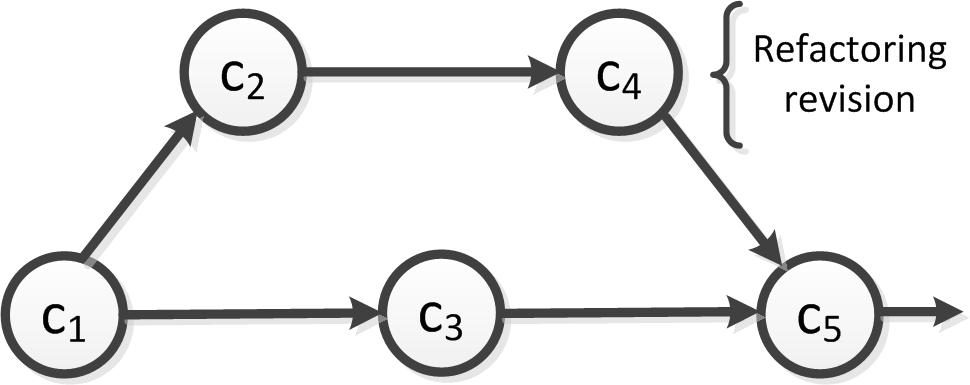
\includegraphics[width=2.5in]{../img/implicit_branche}
	\caption{Exemplo de implicit branches \cite{Tsantalis2013}{}.}
	\label{fig:implicit_brache}
\end{figure}

As refatorações foram detectadas utilizando a técnica proposta Tsantalis et al. \cite{Tsantalis2013}{} que é baseada no algoritmo \texttt{UMLDiff} \cite{Xing:2005:UAO:1101908.1101919}. Tendo em vista a ausência de código compilado foi utilizado uma implementação da técnica com algumas adaptações \cite{Danilo}. A ferramenta proposta Tsantalis et al. é capaz de detectar 11 tipos diferentes de refatoração. Para a refatoração \textit{Mover Classe} a detecção ocorre com base nas seguintes regras definidas por \cite{Biegel:2011:CSM:1985441.1985452}:

\begin{itemize}
	\item Seja $(p,n,m)$ uma tupla tal que $p$ é o pacote que uma classe pertence, $n$ é o nome da classe e $m$ é o conjunto de métodos e campos que compõe a classe.
	\item Seja $t$ uma transação que corresponda uma comparação entre duas revisões sucessivas de um sistema
	\item Seja $C^{+}_{t}$ o conjunto de classes adicionadas na transação $t$
	\item Seja $C^{-}_{t}$ o conjunto de classe removidas na transação $t$
	\item A refatoração é detectado quando as duas condições a seguir são verdadeiras:
		\begin{itemize}
			
			\item $\exists (p,n,m) \in C^{-}_{t}$
			\item $\exists (p^{'},n,m) \in C^{+}_{t}$
		
		\end{itemize}
\end{itemize}

Em resumo a detecção do refatoração \textit{Mover Classes} consiste em verificar se uma classe que previamente existia um em pacote $p$ na versão $v_{1}$ está no pacote $p^{'}$ na versão subsequente $v_{2}$. No estudo empírico de \cite{Tsantalis2013} foi verificado um número baixo de falsos positivos e por consequência uma alta precisão quando utilizado este conjunto de regras na detecção de Mover Classe.

%\subsubsection{Seleção dos \texttt{batching moving} }
%
%Conforme a definição proposta neste trabalho, um  \texttt{batching moving} representa uma movimentação de classe em um número maior do que padrão do sistema. Desta forma, para detectamos este tipo de evento foi necessário avaliar a frequência que a refatoração Mover Classe ocorre nos sistemas em estudo. Neste estudo foi definido que a ocorrência de \texttt{batching moving} é determinada por um total de classe movimentadas que é maior o igual 1.5 vezes a média de ocorrência da refatoração Mover Classe no sistema.



%\subsection{Análise das Mensagens de Commit}
%\label{subsec:analise_commit}
%
%Com o objetivo de analisar se os desenvolvedores reportam que a refatoração Mover Classe teve como objetivo alterar a arquitetura do sistema, foi realizada uma inspeção manual nas mensagens dos commits. Foi avaliado aqueles commits que movimentaram classe um número maior do que 1.5 vezes a média do sistema. Na busca foi avaliado a existência de evidências que a refatoração visava melhorar algum atributo interno do sistema ou ainda adequar a alguma arquitetura previamente definida. 

%\subsection{Pesquisas com os Desenvolvedores}
%\label{subsec:pesquisas_desenvolvedores}


\section{Resultados}
\label{sec:resultados}

Neste seção apresentados os resultados para a questão de pesquisas propostas. Em resumo, este estudo avaliou um total de \textit{52001} diferentes versões de sistemas, do qual foi possível detectar o montante de \textit{35402} refatorações diferente. A Tabela \ref{tab:visao-geral} exibe os valores da média, mediana e desvio padrão da distribuição de Mover Classe entre as diferente versões dos sistemas.

\begin{table}[htb]
	\centering
	\resizebox{\textwidth}{!}{%
		\begin{tabular}{|c|c|c|c|c|c|}
			\hline
			\textbf{Projeto} & \textbf{Total} & \textbf{Média} & \textbf{Mediana} & \textbf{Desvio Padrão} & \textbf{Valor do batching moving} \\ \hline
			clojure          & 64             & 15,5           & 2                & 23,08                  & 23                                \\ \hline
			gradle           & 4253           & 31,3           & 2                & 12,9                   & 46                                \\ \hline
			junit4           & 279            & 12             & 2                & 7,9                    & 18                                \\ \hline
			spring-framework & 1427           & 26             & 2                & 12,5                   & 39                                \\ \hline
		\end{tabular}%
	}
	\caption{Media, Mediana, Desvio Padrão e Valor do batching moving}
	\label{tab:visao-geral}
\end{table}


Do total de refatorações encontrados 17\% era do tipo Mover Classe. A coluna \textit{Mover Classe} exibe o número da refatoração em estudo, bem como o seu percentual, para cada sistema.  A Tabela \ref{tab:estatisticas} detalha estes resultado para cada projeto.


% Please add the following required packages to your document preamble:
% \usepackage{graphicx}
\begin{table}[htb]
	\centering
	\resizebox{\textwidth}{!}{%
		\begin{tabular}{|c|c|c|c|}
			\hline
			\textbf{Projeto} & \textbf{\#Commits} & \textbf{\#Refactorings} & \textbf{\#Mover Classe} \\ \hline
			clojure & 2923 & 522 & 64 (12,3\%) \\ \hline
			gradle & 35593 & 20258 & 4253 (21\%) \\ \hline
			junit4 & 1721 & 1070 & 279 (26,1\%) \\ \hline
			spring-framework & 11764 & 13552 & 1427 (10,5) \\ \hline
			Total & 52001 & 35402 & 6023 (17\%) \\ \hline
		\end{tabular}%
	}
	\caption{Estatísticas dos Sistemas Analisados}
	\label{tab:estatisticas}
\end{table}

\subsection{Com qual frequência a refatoração Mover Classe tem por objetivo alterar a arquitetura do sistema (\texttt{batching moving})?}

As Figuras \ref{fig:resultado-clojure}, \ref{fig:resultado-gradle}, \ref{fig:resultado-junit}, \ref{fig:resultado-spring} exibem a frequência da refatoração Mover Classe nos sistemas estudados. Por exemplo, na Figura \ref{fig:resultado-clojure} é possível verificar a ocorrência de uma (01) refatoração do tipo Mover Classe onde um total de 54 itens foram movidos. Da mesma forma, a Figura \ref{fig:resultado-gradle} demonstra os resultados do sistema \texttt{gradle} em que na maior parte das revisões o máximo de classe movidas chegam à 40 itens.


\begin{figure}[htb]
\centering
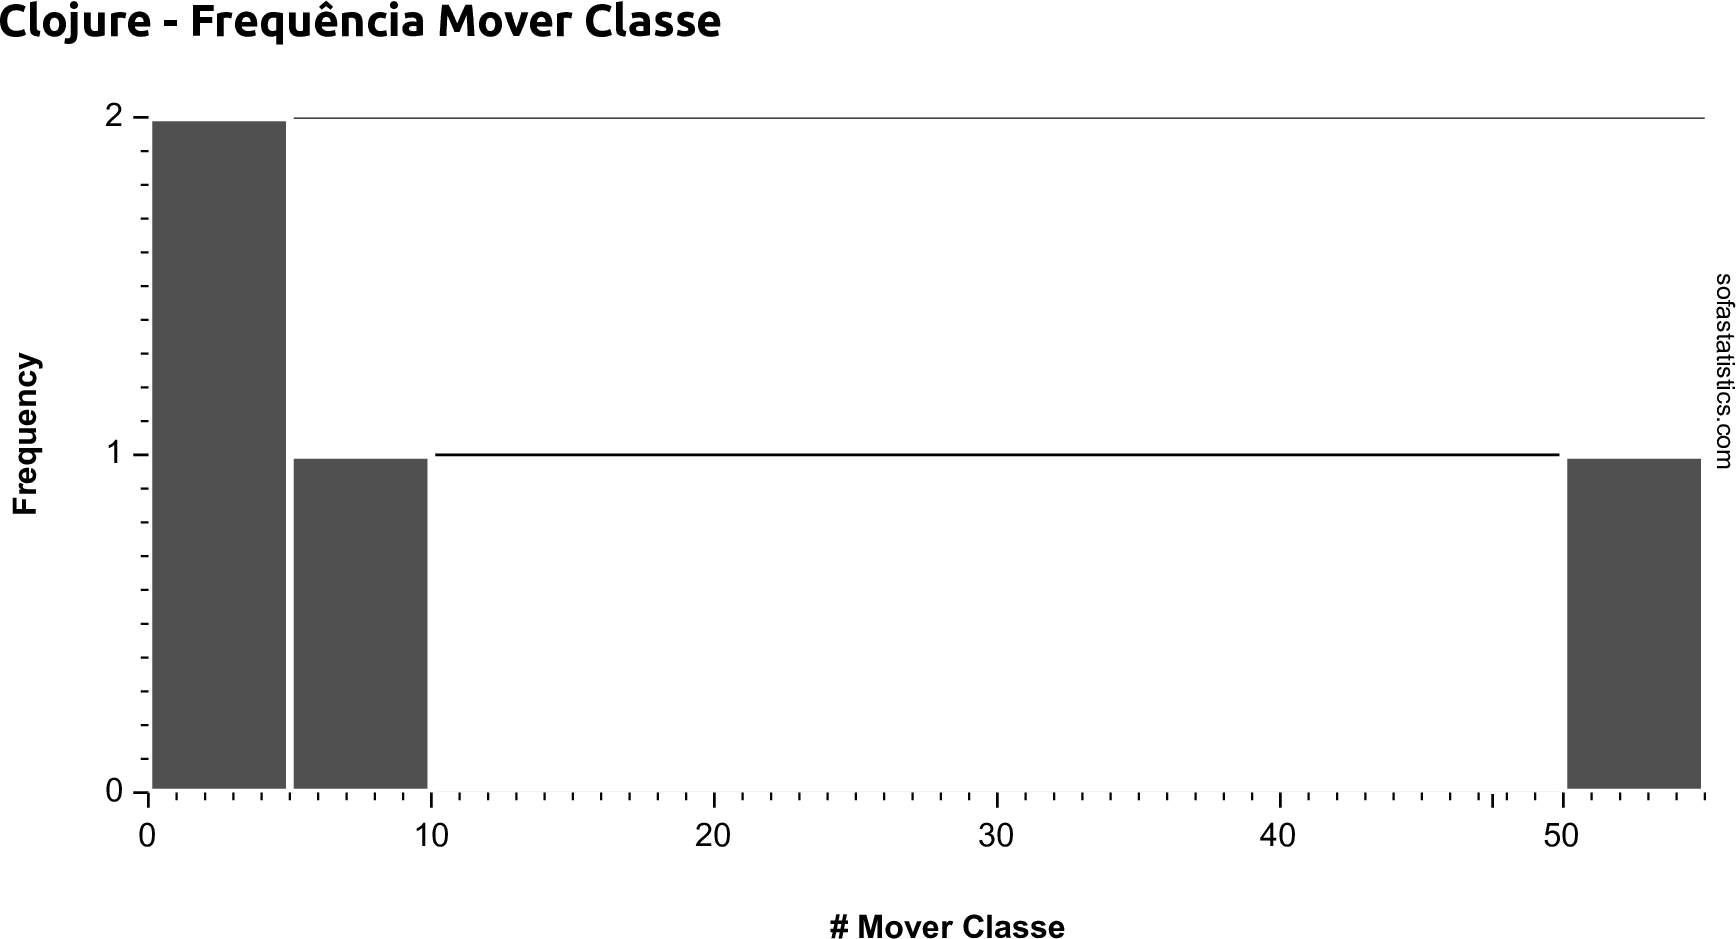
\includegraphics[width=0.9\linewidth]{../img/0006_Histogram_Clojure_Frequencia_Mover_Classe}
	\caption{Clojure - Frequência de Mover Classe}
\label{fig:resultado-clojure}
\end{figure}

\begin{figure}[htb]
	\centering
	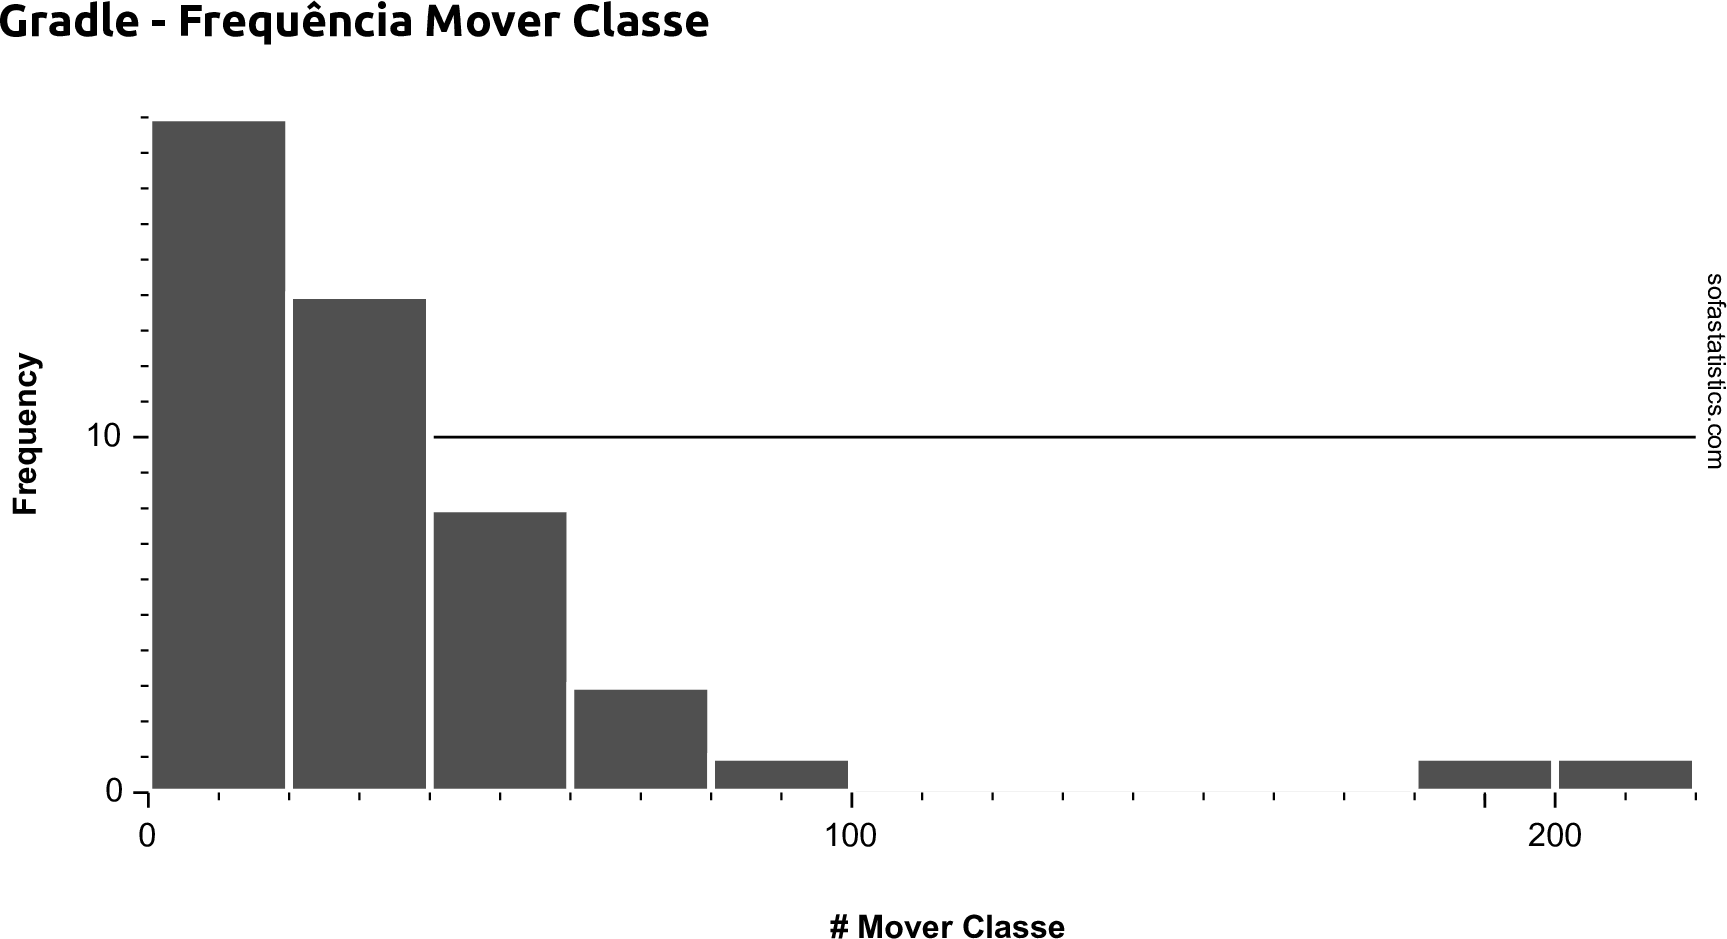
\includegraphics[width=0.9\linewidth]{../img/0008_Histogram_Gradle_Frequencia_Mover_Classe}
	\caption{Gradle - Frequência de Mover Classe}
	\label{fig:resultado-gradle}
\end{figure}

É possível observar uma tendência de um menor número de classe sendo movimentadas, contudo, em uma maior frequência. Não obstante, ocorre alguns eventos em que um grande número de classe são movidas, como por exemplo, no sistema \texttt{gradle} onde foi detectado a refatoração Mover Classe para mais de 200 classes. Este tipo de ação possivelmente causa alteração na arquitetura dos sistema. 

A fim de responder a questão de pesquisa proposta é exibida a Tabela \ref{tab:resultados-frequencias} a frequência de ocorrência de movimentação de classes em um número maior ou igual a coluna \textit{Classe Movidas}. Por exemplo, no projeto \texttt{junit4} cerca de 24\% do Mover Classe ocorre com 5 ou mais classes. Em média, cerca de 27\% das movimentações de classe foram com 5 ou mais classe.

\begin{table}[]
	\centering
	\resizebox{\textwidth}{!}{%
		\begin{tabular}{|c|c|c|c|c|c|}
			\hline
			\textbf{Classe Movidas} & \textbf{clojure} & \textbf{gradle} & \textbf{junit4} & \textbf{spring-framework} & \textbf{Média} \\ \hline
			\textit{5} & 0,40 & 0,208 & 0,237 & 0,271 & 0,279 \\ \hline
			\textit{10} & 0,20 & 0,063 & 0,136 & 0,136 & 0,13375 \\ \hline
			\textit{15} & 0,20 & 0,047 & 0,085 & 0,104 & 0,109 \\ \hline
			\textit{20} & 0,20 & 0,027 & 0,068 & 0,086 & 0,09525 \\ \hline
			\textit{30} & 0,20 & 0,027 & 0,017 & 0,054 & 0,0745 \\ \hline
			\textit{40} & 0,20 & 0,021 & 0,017 & 0,036 & 0,0685 \\ \hline
			\textit{50} & 0,20 & 0,010 & - & 0,018 & - \\ \hline
			\textit{60} & - & 0,008 & - & 0,009 & - \\ \hline
			\textit{70} & - & 0,007 & - & 0,009 & - \\ \hline
			\textit{80} & - & 0,005 & - & 0,005 & - \\ \hline
			\textit{90} & - & 0,002 & - & 0,005 & - \\ \hline
			\textit{100} & - & 0,002 & - & 0,005 & - \\ \hline
			\textit{150} & - & 0,002 & - & - & - \\ \hline
			\textit{200} & - & 0,001 & - & - & - \\ \hline
		\end{tabular}%
	}
	\caption{Frequência da Movimentação das Classes}
	\label{tab:resultados-frequencias}
\end{table} 


Os resultados da Tabela \ref{tab:resultados-frequencias} demonstram que a frequência de \texttt{batching moving} é relativamente baixa nos sistemas analisados. Se consideramos um limiar  (threshold) de \textit{40} classe movidas por revisão, \textit{a ocorrência média é de 6\%}. Todavia, da baixa frequência foi possível detectar este tipo padrão em todo os sistemas analisados.

\begin{figure}[htb]
	\centering
	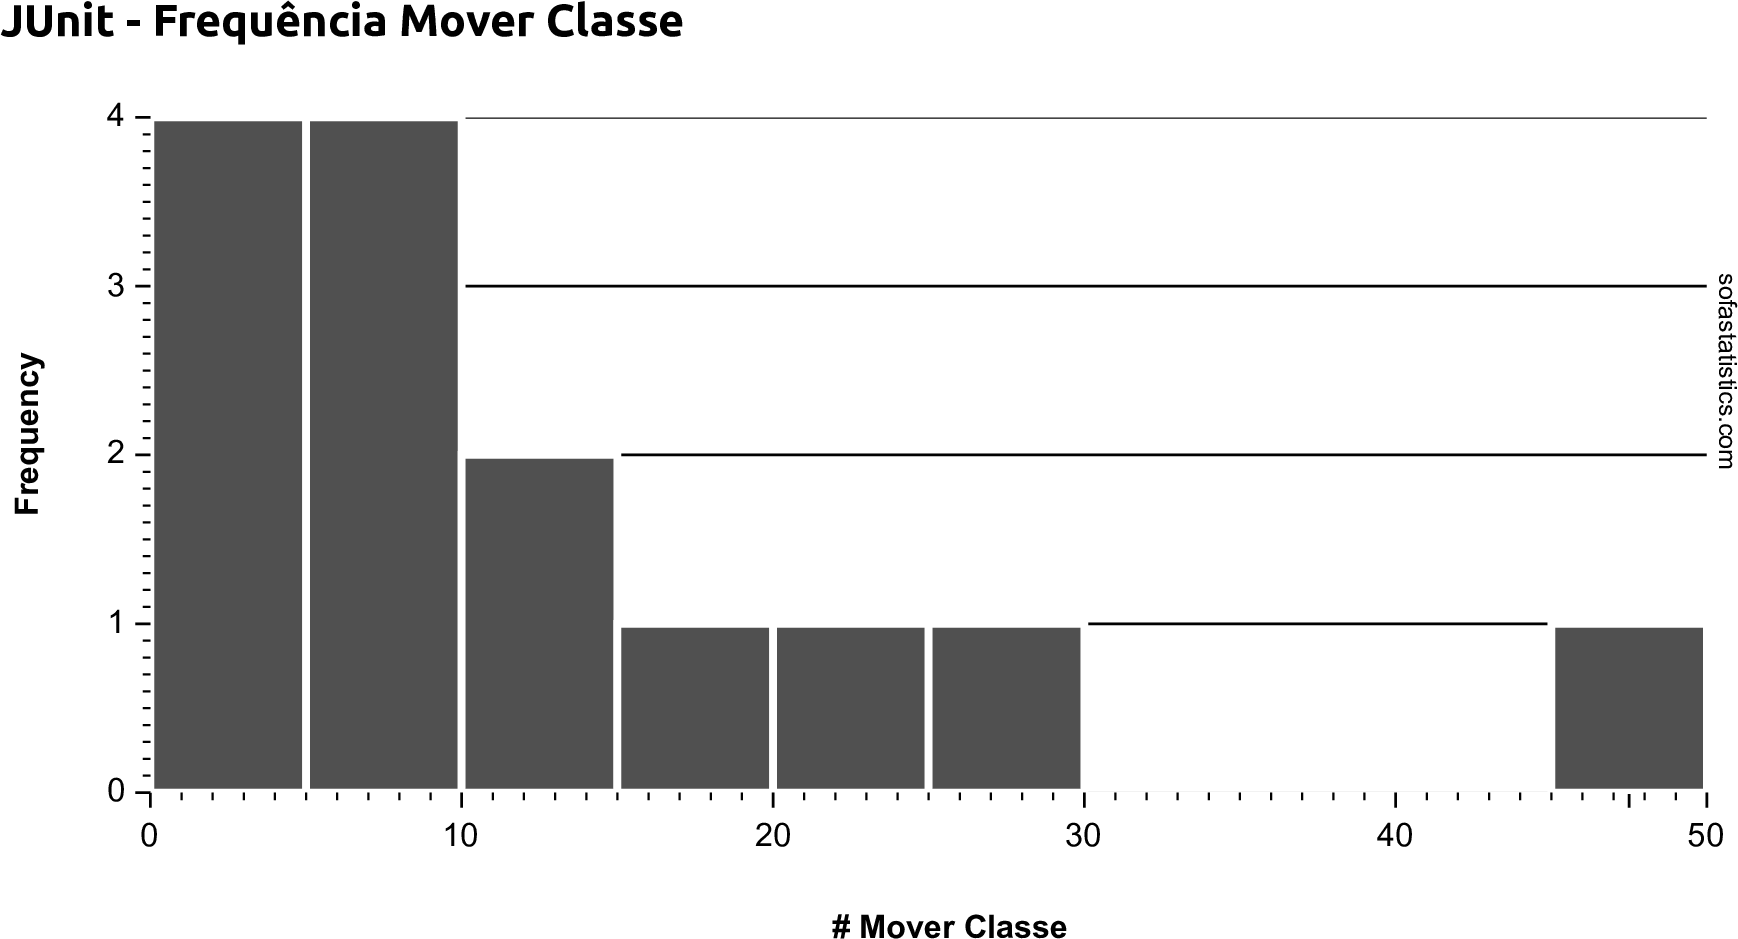
\includegraphics[width=0.9\linewidth]{../img/0014_Histogram_JUnit_Frequencia_Mover_Classe}
	\caption{JUnit - Frequência de Mover Classe}
	\label{fig:resultado-junit}
\end{figure}


\begin{figure}[htb]
	\centering
	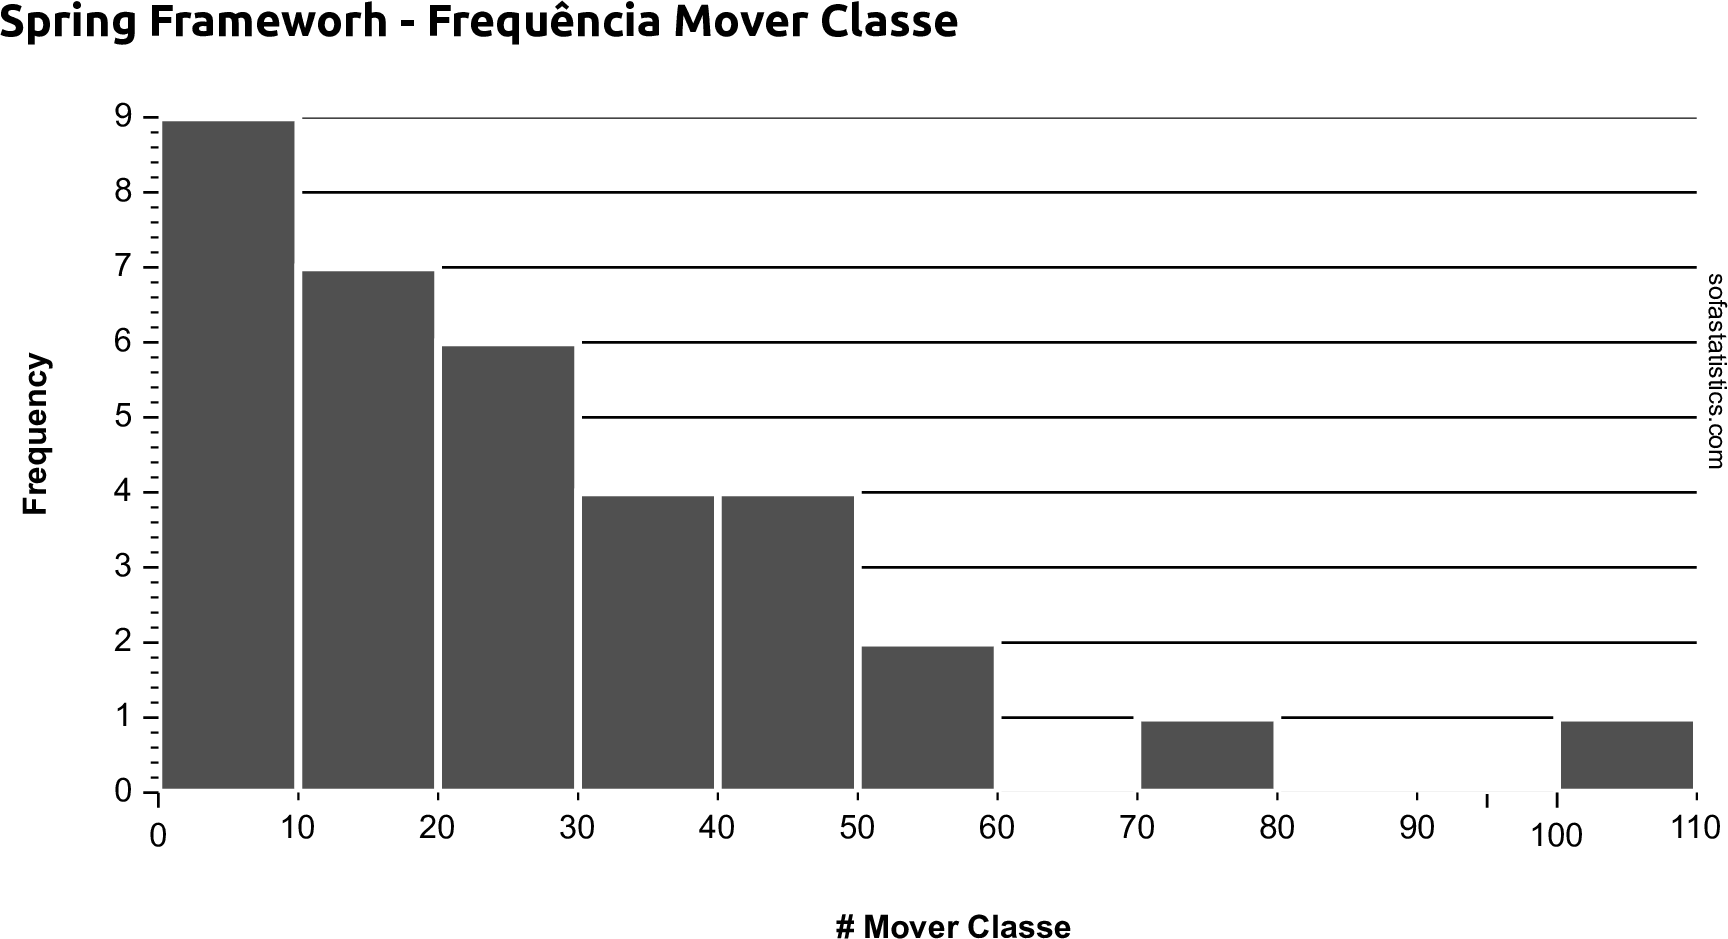
\includegraphics[width=0.9\linewidth]{../img/0015_Histogram_Spring_Frameworh_Frequencia_Mover_Classe}
	\caption{Spring Framework - Frequência de Mover Classe}
	\label{fig:resultado-spring}
\end{figure}

\section{Ameaças à Validade}
\label{sec:ameacas}

As ameaças à validade de qualquer estudo podem surgir de diversas formas e de diferentes direções. A \textit{Ameaça Interna} avalia se o tratamento utilizado produziu algum efeito, ou seja, se a variável independente realmente causa mudanças observáveis na variável dependente examinada \cite{7230299}. Neste estudo existem pelos menos as seguintes ameças internas:

\begin{itemize}
	\item A precisão dos resultados obtidos dependem do quão precisa é a ferramenta de detecção utilizada. Desta forma, existe a possibilidade de ocorrência de falso negativos, pois não ha uma estimativa confiável da revocação da ferramenta. 
	
	\item Não é possível definir um limiar (threshold) no qual podemos afirmar que a quantidade de classe movidas estão alterando a arquitetura do sistema. Assim a determinação \texttt{batching moving} dependerá da quem está analisando o sistema.
		
\end{itemize}
 
\textit{Ameaça Externa} é uma análise crítica do quanto os resultados obtidos em um estudo podem ser generalizados. Neste trabalho, a análise recai sobre os critérios de seleção dos sistemas, em especial os que estão listados a seguir:
 
 \begin{itemize}
 	
  \item O total de sistemas escolhidos não permitem a generalização dos resultados.
  
  \item  Os sistema escolhidos pertencem a única linguagem de programação, desta forma, poderíamos esperar outros resultados quando utilizados software desenvolvidos em outras linguagens.
  
  \item Os sistemas analisados são todos de uma  única fonte (\texttt{GitHub}). Os resultados podem ser diferentes para sistemas comerciais ou desenvolvidos em outras comunidades de desenvolvimento.
  
 \end{itemize}

\section{Trabalhos Relacionados}
\label{sec:trabalhos-relacionados}

Apesar de sua reconhecida importância os padrões de uso do refactoring é ainda pouco conhecido. Além disso, a sua aplicação de forma manual pelos desenvolvedores é bastante custosa. Afim de preencher estas lacunas diversos trabalhos vêm sendo propostos.  No trabalho de \cite{Dig:2009:RSJ:1555001.1555054}{} é apresentado uma ferramenta visa facilitar o desenvolvimento de aplicações multi-threads em java por meio de refactorings automatizados na biblioteca \textit{java.util.concurrent}{}. Os resultados demostraram que a ferramenta conseguiu detectar oportunidades de refatoração que os desenvolvedores negligenciaram, ao mesmo tempo que conseguir uma boa taxa de conversão de código. 

Em \cite{icpc2014}, Silva et. al propõe-se uma ferramenta visando automatizar a recomendação  refactorings. O estudo apresenta uma nova abordagem para identificar e ranquear oportunidades de \textit{Extract Methods} de modo a ser automatizado nas IDE's. Por meio de um estudo exploratório foi possível verificar que a ferramenta atingiu um percentual de 48\% de precisão ao avaliar uma amostra de 81 extracts methods artificialmente gerados. 

Seguindo esta mesma linha, o trabalho de \cite{wcre2013a} propõe uma ferramenta de recomendação de \textit{Move Method}{} refactorings utilizando uma técnica denominada \textit{Dependency Sets}{}. A partir da premissa que ``métodos em classes bem desenhadas geralmente estabelecem dependências entre tipos semelhantes" os autores avaliam a similaridade das dependências estabelecidas por um método com os demais em sua classe com os demais métodos das outras classes no sistema. Neste sentido é possível ranquear as classe  e por conseguinte recomendar a mudança do método para uma das classes que possui maior similaridade que sua classe atual. Nos testes efetuados esta técnica se mostrou superior àqueles apresentadas pelo \textit{JDeodorant\footnote{http://www.jdeodorant.com/}}, um sistema de recomendações de move method bem conhecido. Na mesma linha de pesquisa, contudo com o foco bem distinto, em \cite{Feldthaus11tool-supportedrefactoring} temos uma proposta de refatoração automatizada de uma linguagem de tipagem dinâmica. Percebe-se na literatura uma concentração de pesquisas sobre refactoring em linguagens de tipagem estática, tais como Java, para as quais é possível tirar vantagem de informações por meio da análise estática do código. Em contrapartida, refatoração para linguagens dinâmicas como JavaScript é complicado devido aos identificadores da linguagem serem resolvidas em tempo de execução. A fim de preencher esta lacunas os autores apresentam uma ferramenta para recomendar refactorings em códigos escritos em JavaScript. Apesar do limitado conjunto de refatorações suportados pela ferramenta, ela abre o caminho para o desenvolvimento de técnicas de recomendação de refactorings em linguagem de tipagem dinâmica.

Um segundo grupo de trabalho na sobre refactorings visa avaliar e entender os padrões de uso desta técnica. Podemos dividir estes estudos em duas abordagens principais: aqueles que coletam os dados diretamente da IDE, através de um plugin por exemplo; outra que analisam diferentes versões de um código, por meio de um Sistema de Controle de Versão, a fim de detectar padrões. Em  \cite{Robbes:2007:MCS:1268983.1269029} é proposto um repositório alternativo de informações ao qual coleta mudanças incrementais do sistema em estudo diretamente da IDE do programado. Com base nos dados coletados os autores avaliam os padrões de refactoring em dois casos de estudos, além de comparar o resultados com clássica abordagem da coleta de refactorings em CVS. 

Na mesma linha \cite{NegaraETAL2013ManualRefactorings} se propões a analisar as diferenças entre refactorings manual e automáticos, ou seja, entre aqueles realizados diretamente pelo desenvolvedor e aqueles produzidos por meio de uma funcionalidade da IDE. Para tanto, os autores desenvolveram um plugin que coletou um total de 1.520 de trabalho de 23 programadores. O trabalho indicou que em média 30\% dos refactoring não chegam aos CVS's. A principal contribuição deste tipo de enfoque é permitir analisar separadamente os padrões de rafactoring manual e automático. Contudo, como os dados são coletados diretamente da IDE, o possível overhead gerado pode desmotivar a participação de um maior número de desenvolvedores.  Outra limitador é a pouca abrangência deste tipo de abordagem, tendo em vista que o pesquisador necessitar criar um novo plugin para cada tipo de linguagem/paradigma estudado \cite{Robbes:2007:MCS:1268983.1269029}.

Em \cite{Xing:2005:UAO:1101908.1101919} é apresentado o \textit{UMLDiff},  um algoritmo capaz de detectar automaticamente alterações estruturais entre duas versões de um software orientado a objetos. Basicamente ele toma como entrada dois diagramas de classe de um sistema e produz uma ``árvore de mudanças" que registra as alterações realizadas no software. Por conta de sua capacidade de exibir as alterações estruturais entre duas versões do sistema, o \textit{UMLDiff} é utilizado com algoritmo base para detecção de refactorings \cite{Tsantalis:2013:MES:2555523.2555539}{}. Este trabalha utiliza este algoritmo como base para detecção de refactorings.

\section{Conclusão}
\label{sec:conclusao}

Este trabalho se propôs em analisar o fenômeno \texttt{batching moving} e seu efeito na arquitetura de software. Apesar da sua baixa frequência, chegando em alguns em cerca de 6\% do total, este tipo de ação foi detectado em todos os sistemas analisados. Neste sentido, as ferramentas podem ser melhoradas para dar um maior suporte a este tipo de operação. Não obstante, os estudo que avaliam a evolução da arquitetura do software devem ter uma maior atenção a este fenômeno com objetivo de entender quais as motivações de um desenvolver mudar diversas classes do sistema, como por exemplo, mais de 200 classe em uma revisão em uma mesma revisão como demostrado neste estudo.

Como possíveis extensões deste trabalho pretende-se analisar o texto do \textit{log de commit} dos possíveis \texttt{batching moving} com o objetivo de avaliar qual a frequência que o desenvolvedor informa que a refatoração teve por objetivo alterar a arquitetura do sistema. Um novo ponto de ampliação do escopo deste estudo é verificar, mediante uma pesquisa com os desenvolvedores, se Mover Classe foi efetivamente utilizado visando alterar a arquitetura dos sistema.

\bibliographystyle{sbc}
\bibliography{../bib/paper-arqsw}

\end{document}
